% ═══════════════════════════════════════════════════════════════════
% Figure captions for:
% "Football as a Partially Observable Bioreactor:
%  Backward Biomechanical Accounting via the Ball Observation Operator"
% ═══════════════════════════════════════════════════════════════════

\begin{figure*}[!htbp]
    \centering
    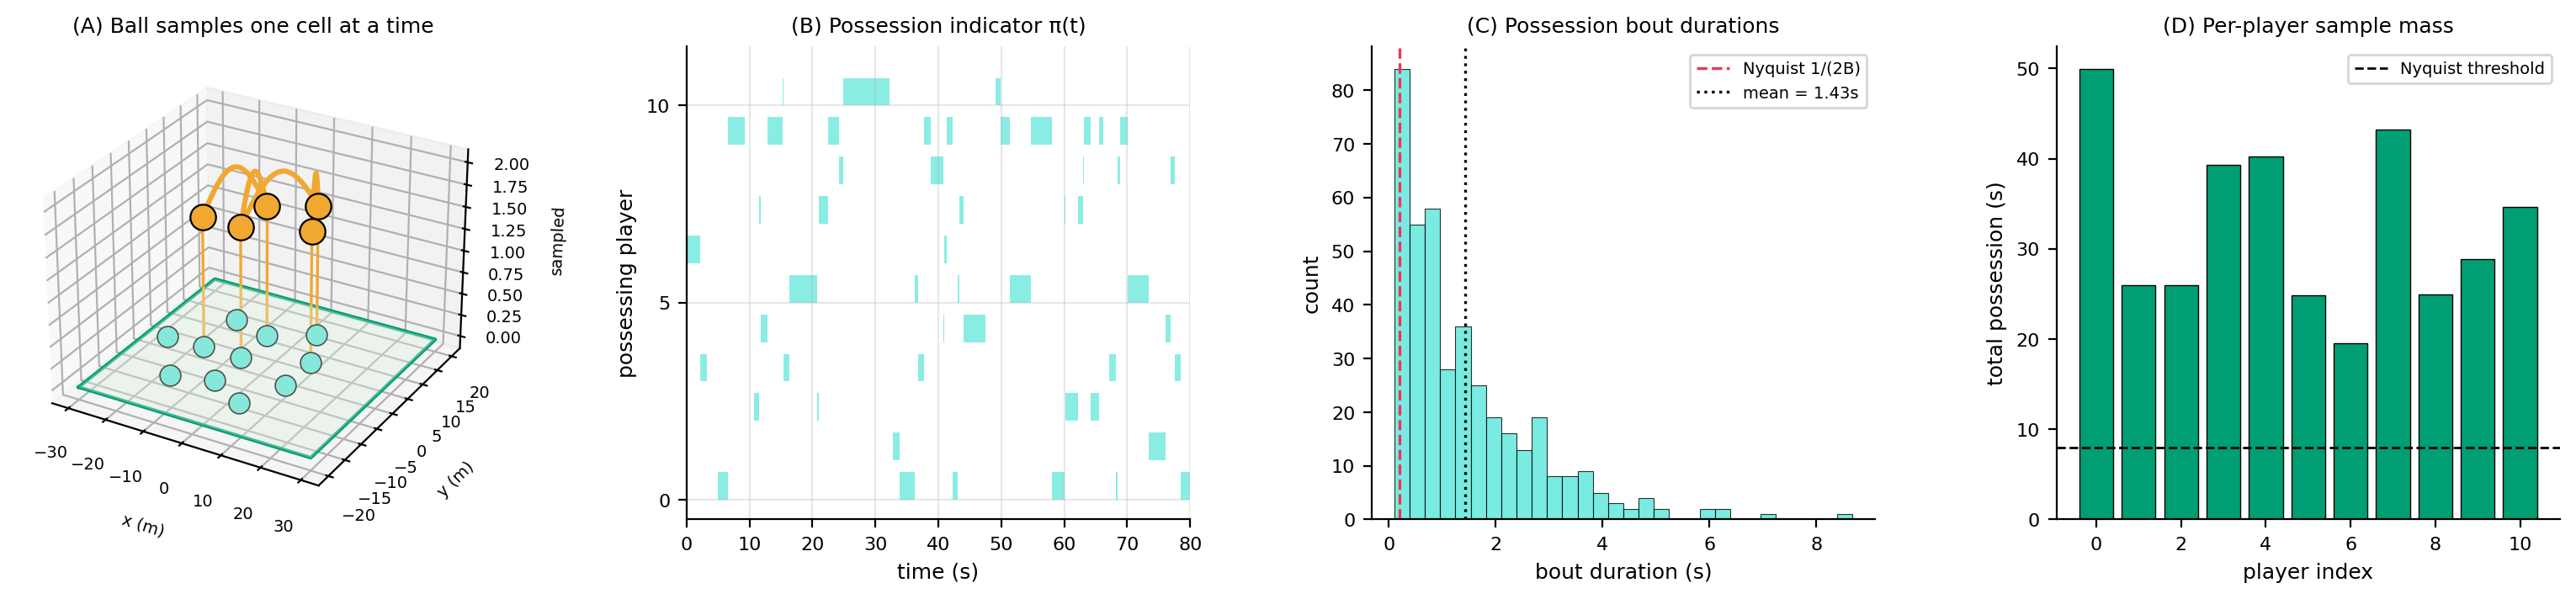
\includegraphics[width=\textwidth]{figures/panel1_observation_operator.png}
    \caption{\textbf{Observation-operator sampling on the pitch-bioreactor.}
    (\textbf{A})~Three-dimensional rendering of a schematic football pitch
    with eleven player positions in a 4--3--3 formation (cyan) and the
    ball trajectory (amber) lifted into a vertical ``sampled cell''
    coordinate. The ball touches one player at a time at high fidelity,
    rising into the sampled-cell coordinate at each contact and travelling
    between cells in arcs; the remaining ten cells evolve at $z=0$ in the
    bioreactor's bulk and are not directly sampled.
    (\textbf{B})~Possession indicator $\pi(t)$ over a 80-second window.
    Each cyan block is a possession bout of a single player; the grey
    gaps mark $\pi(t)=*$ (ball in flight or unpossessed). The function
    is piecewise constant, with bout boundaries triggering re-targeting
    of the high-fidelity sample channel.
    (\textbf{C})~Distribution of possession-bout durations across 400
    simulated bouts. The mean bout duration is $1.43$~s, well above the
    Nyquist threshold $1/(2B)=0.20$~s for a biomechanical signal of
    bandwidth $B=2.5$~Hz (red dashed line), confirming that typical
    elite-football bouts Nyquist-sample gait biomechanics for any player
    whose touches are not micro-deflections.
    (\textbf{D})~Per-player total possession time over a single match,
    coloured by the Nyquist threshold (green: above 8~s, red: below).
    The accounting framework requires sufficient cumulative sample mass
    to reconstruct each player's biomechanical trajectory; players with
    insufficient touches (defenders rarely on the ball) rely more
    heavily on the ambient observation channel.}
    \label{fig:obsop}
\end{figure*}


\begin{figure*}[!htbp]
    \centering
    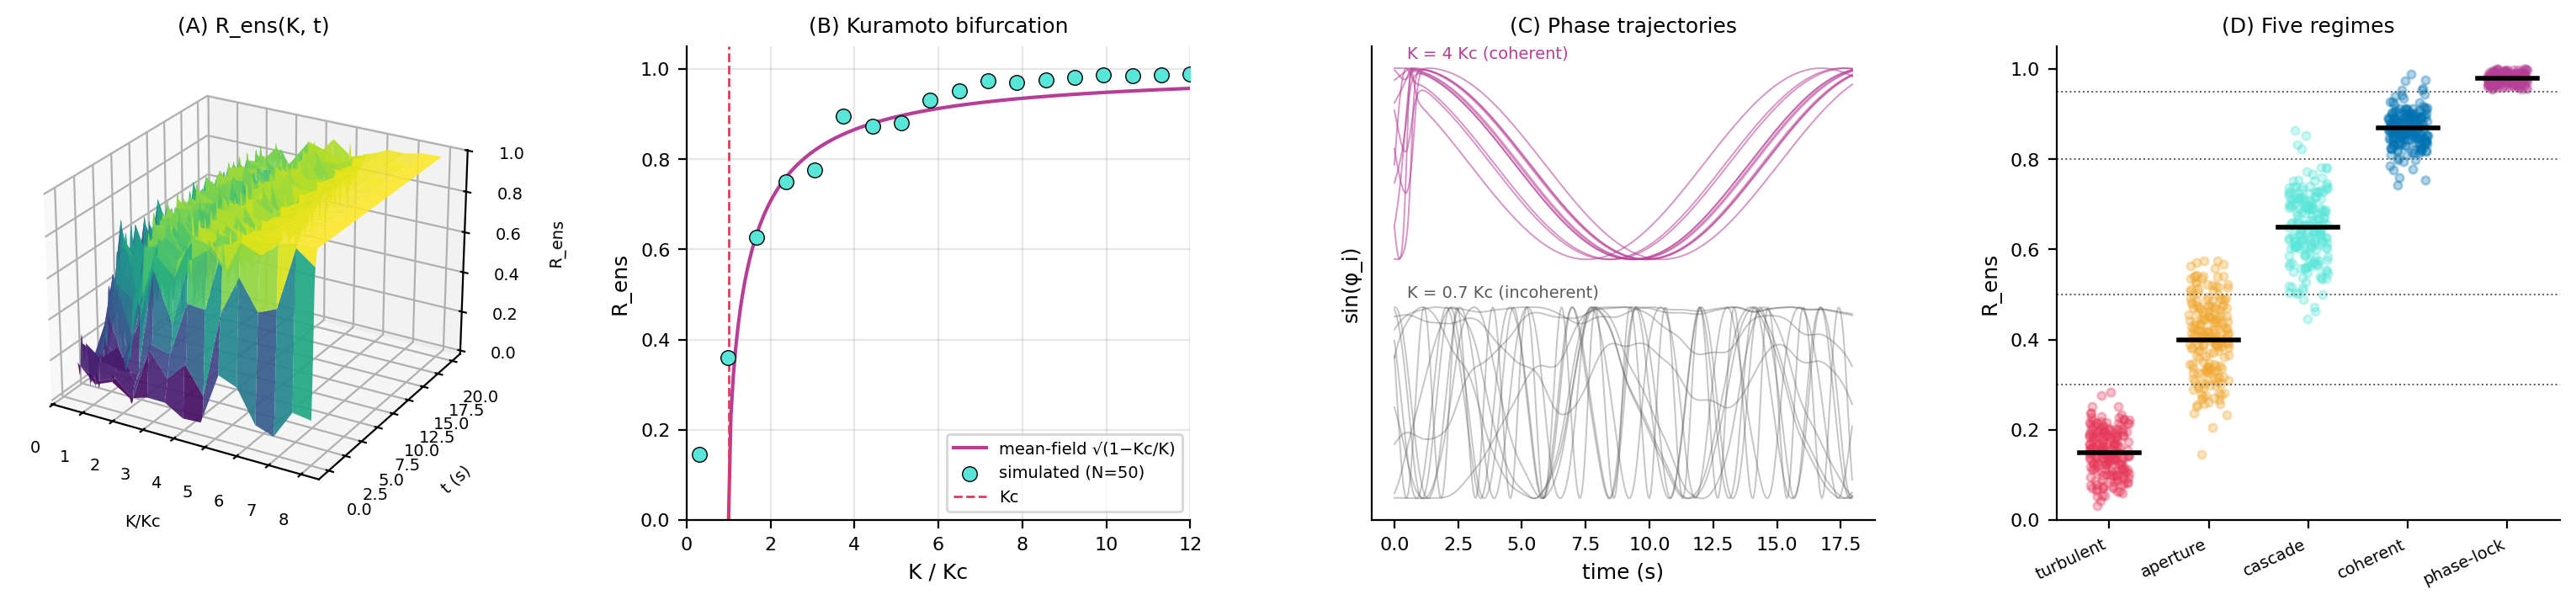
\includegraphics[width=\textwidth]{figures/panel2_bifurcation.png}
    \caption{\textbf{Kuramoto bifurcation and the five coherence regimes.}
    (\textbf{A})~Three-dimensional surface of the team order parameter
    $R_{\mathrm{ens}}(K, t)$ across a sweep of coupling strengths
    $K/K_{c}\in[0.5,8]$ and time $t\in[0,20]$~s, for an ensemble of
    $N=40$ Cauchy-distributed oscillators. The surface rises from the
    incoherent floor at low $K$ to a fully synchronised plateau at high
    $K$, with the bifurcation at $K=K_{c}=2\gamma$ visible as the steep
    ridge.
    (\textbf{B})~Equilibrium order parameter $R_{\mathrm{ens}}$ versus
    $K/K_{c}$ for $N=50$ simulated ensembles (cyan dots) against the
    mean-field prediction $R^{*}=\sqrt{1-K_{c}/K}$ (violet line). The
    bifurcation at $K=K_{c}$ (red dashed) separates the incoherent
    state ($R\approx 0$) from the partially phase-locked state
    ($R>0$); the simulated curve matches the mean-field prediction
    above threshold within finite-$N$ tolerance.
    (\textbf{C})~Sinusoidal phase trajectories $\sin(\phi_i(t))$ for
    eleven oscillators at sub-critical ($K=0.7\,K_{c}$, grey) and
    super-critical ($K=4\,K_{c}$, violet, offset) coupling. The
    sub-critical trajectories drift independently; the super-critical
    trajectories synchronise to a common envelope, illustrating the
    team-template emergence at coherent coupling.
    (\textbf{D})~Coherence regime classification. Each of the five
    operational regimes (turbulent, aperture, cascade, coherent,
    phase-lock) appears as a horizontal jitter scatter of $200$
    sample points at its centre $R$ value with the regime mean marked
    by the black bar. Dashed grey lines at $R\in\{0.30, 0.50, 0.80,
    0.95\}$ delineate the regime boundaries.}
    \label{fig:bifurcation}
\end{figure*}


\begin{figure*}[!htbp]
    \centering
    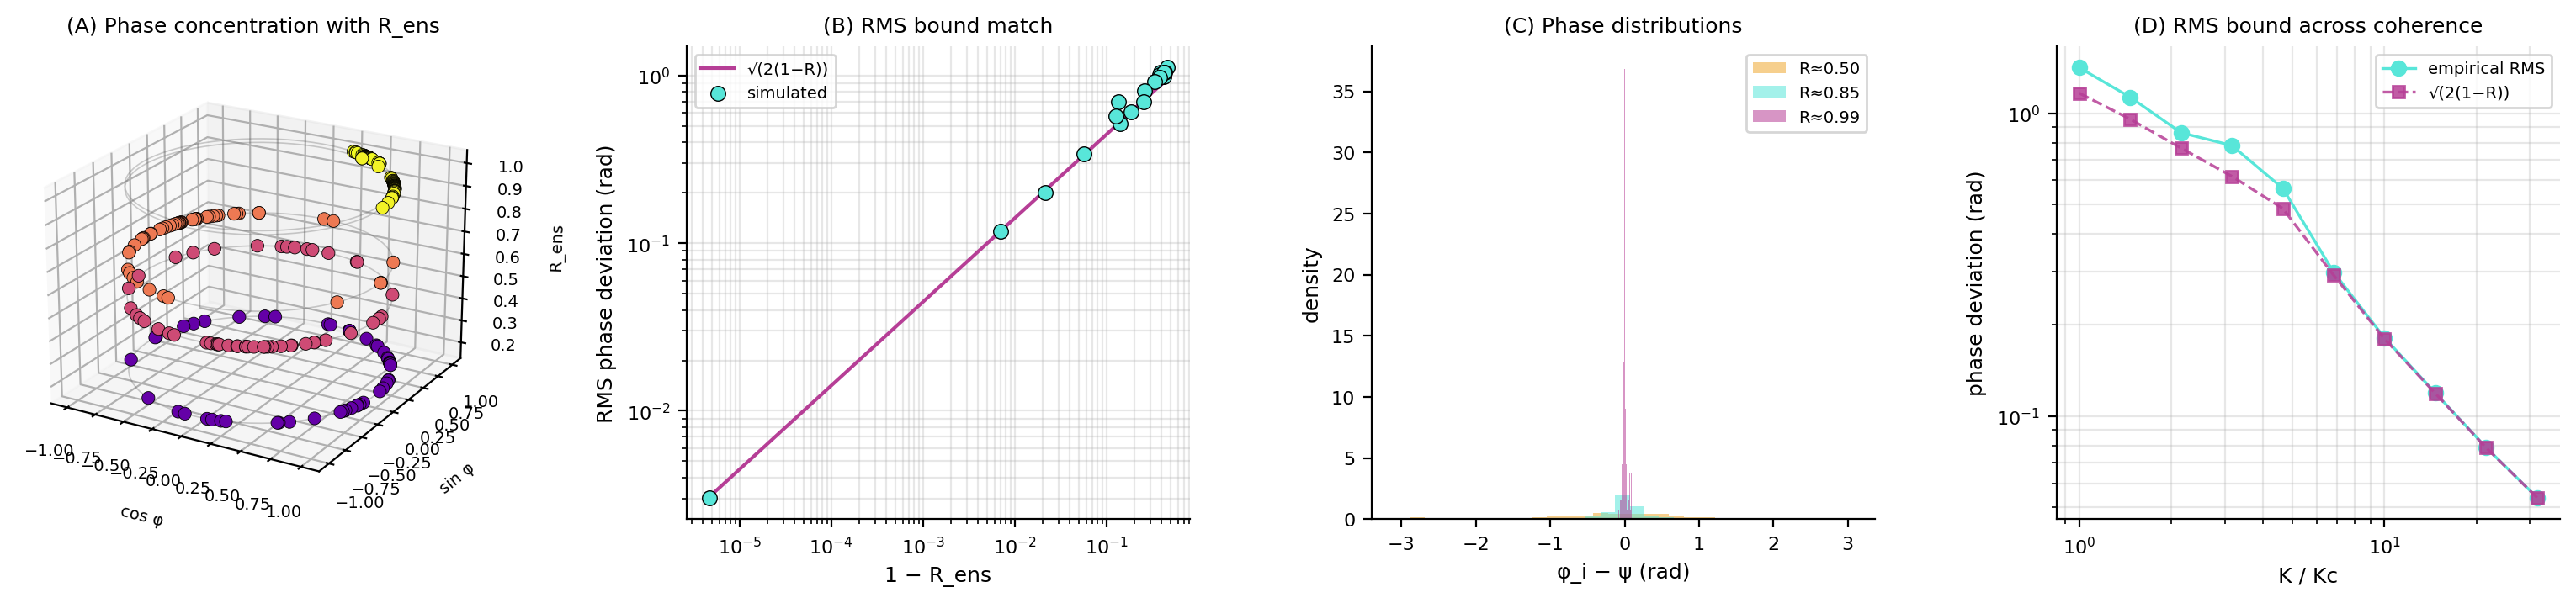
\includegraphics[width=\textwidth]{figures/panel3_templating.png}
    \caption{\textbf{Templating threshold: the team is one template only
    when the phase distribution is concentrated.}
    (\textbf{A})~Three-dimensional rosette: 50 oscillator phases plotted
    on a unit circle (cos\,$\phi$, sin\,$\phi$) at five values of
    $R_{\mathrm{ens}}$ stacked vertically. At low $R_{\mathrm{ens}}$
    (bottom) the phases are uniformly distributed around the circle;
    at high $R_{\mathrm{ens}}$ (top) they concentrate at a single mean
    phase. The geometric concentration is the operational meaning of
    ``one collective body.''
    (\textbf{B})~Empirical RMS phase deviation versus $1-R_{\mathrm{ens}}$
    on log--log axes. The theoretical bound $\sqrt{2(1-R_{\mathrm{ens}})}$
    (violet line) and the simulated values (cyan dots) coincide to
    machine precision across four decades of $1-R_{\mathrm{ens}}$,
    verifying the rigorous RMS form of the templating threshold theorem.
    (\textbf{C})~Density-normalised phase distributions at three
    $R_{\mathrm{ens}}$ levels (0.50 amber, 0.85 cyan, 0.99 violet).
    The distributions narrow continuously as $R_{\mathrm{ens}}$
    approaches unity, demonstrating that the team-template
    approximation becomes increasingly tight in the phase-locked regime.
    (\textbf{D})~Empirical RMS phase deviation (cyan) and theoretical
    bound $\sqrt{2(1-R_{\mathrm{ens}})}$ (violet) across the coupling
    range $K/K_{c}\in[1, 32]$. Both quantities span more than a decade
    and track each other across the full range, confirming that the
    bound is tight throughout the coherent and phase-locked regimes.}
    \label{fig:templating}
\end{figure*}


\begin{figure*}[!htbp]
    \centering
    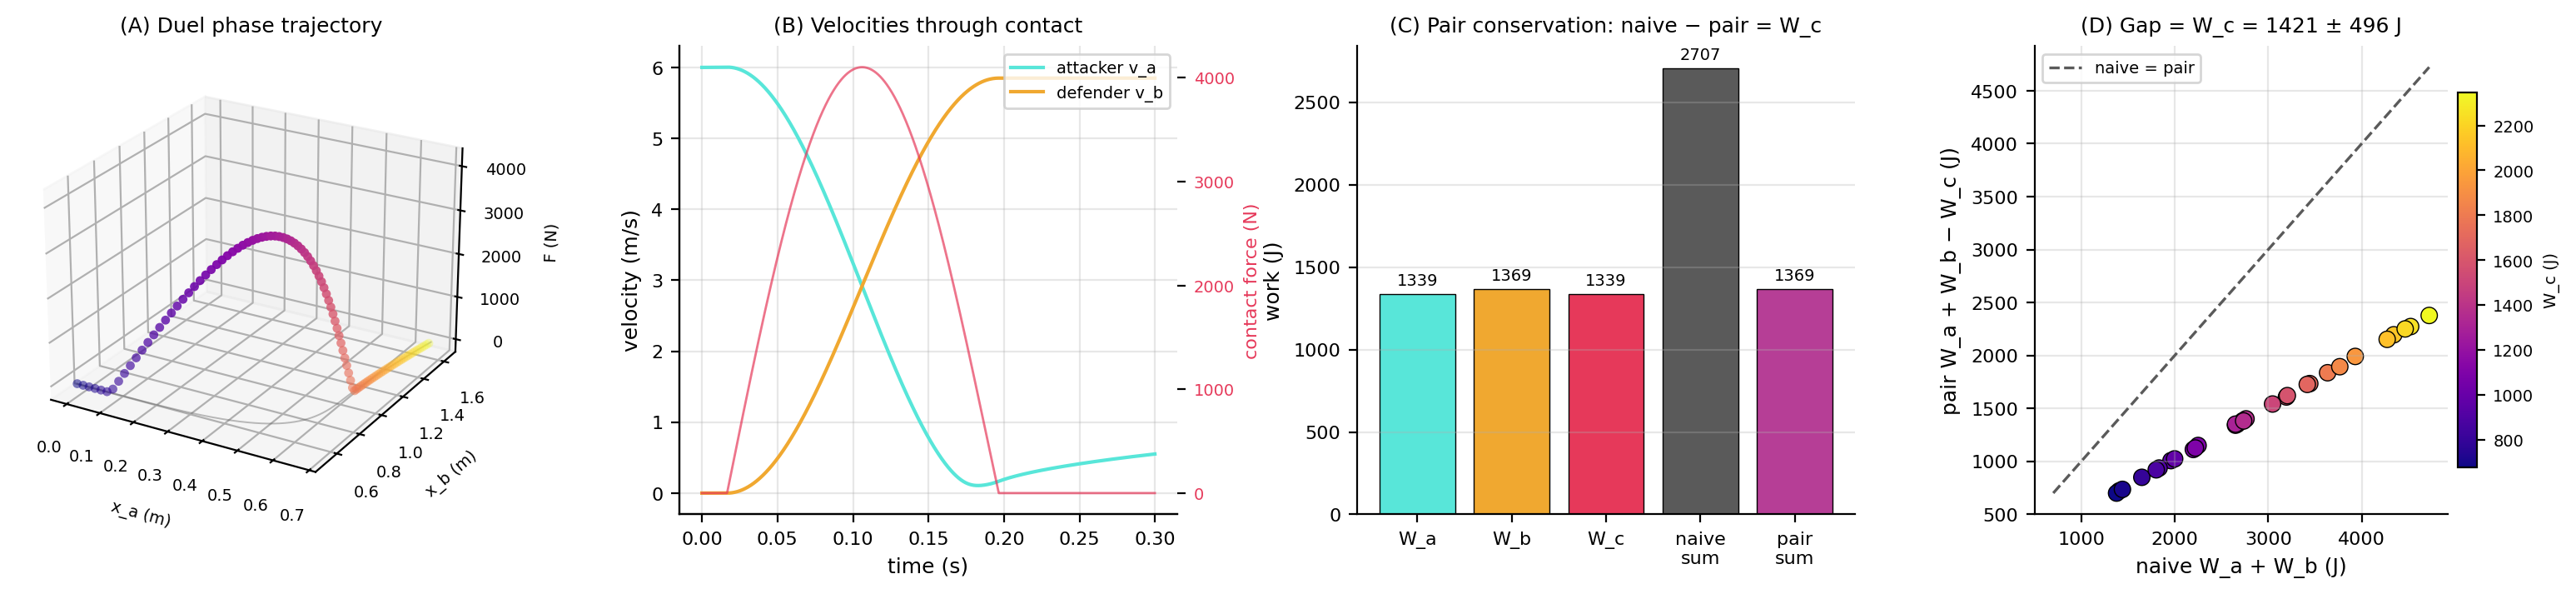
\includegraphics[width=\textwidth]{figures/panel4_duels.png}
    \caption{\textbf{Duels as cognate oscillator pairs and the pair
    conservation of contact load.}
    (\textbf{A})~Three-dimensional phase trajectory of a single duel:
    attacker position $x_{a}$, defender position $x_{b}$, and contact
    force $F(t)$ over a $0.30$~s contestation window. Coloured points
    are sampled along the trajectory by time (plasma colourmap); the
    grey shadow at $F=0$ projects the spatial dynamics. The trajectory
    rises from a no-contact state through a peak contact force and
    relaxes back as the bodies separate.
    (\textbf{B})~Velocities of attacker ($v_{a}$, cyan) and defender
    ($v_{b}$, amber) through the duel, with the contact force
    superimposed on a secondary axis (red). The attacker decelerates
    and the defender accelerates symmetrically during the contact peak,
    illustrating the co-determination of the two cognate halves: neither
    velocity profile is meaningful without the other.
    (\textbf{C})~Pair conservation of contact load. The five bars
    show $|\Delta KE_{a}|$ (cyan), $|\Delta KE_{b}|$ (amber), the
    contact-transferred work $W_{c}$ (red), the naive per-body sum
    $W_{a}+W_{b}$ (grey, double-counts the contact transfer), and the
    pair sum $W_{a}+W_{b}-W_{c}$ (violet). The naive sum exceeds the
    correct pair sum by exactly $W_{c}$, demonstrating that booking
    duels at the pair level (Theorem~4.3) avoids the
    contact-double-counting error of independent per-player accounting.
    (\textbf{D})~Scatter of naive sum versus pair sum across $30$
    randomised duels (varied initial velocities, masses, contact
    stiffness, and metabolic inputs). Points fall along a line
    parallel to but below the identity diagonal, with the
    perpendicular offset equal to $W_{c}$ (colour-encoded); the
    mean gap is $1421\pm 496$~J. The systematic offset is the
    framework's prediction.}
    \label{fig:duels}
\end{figure*}


\begin{figure*}[!htbp]
    \centering
    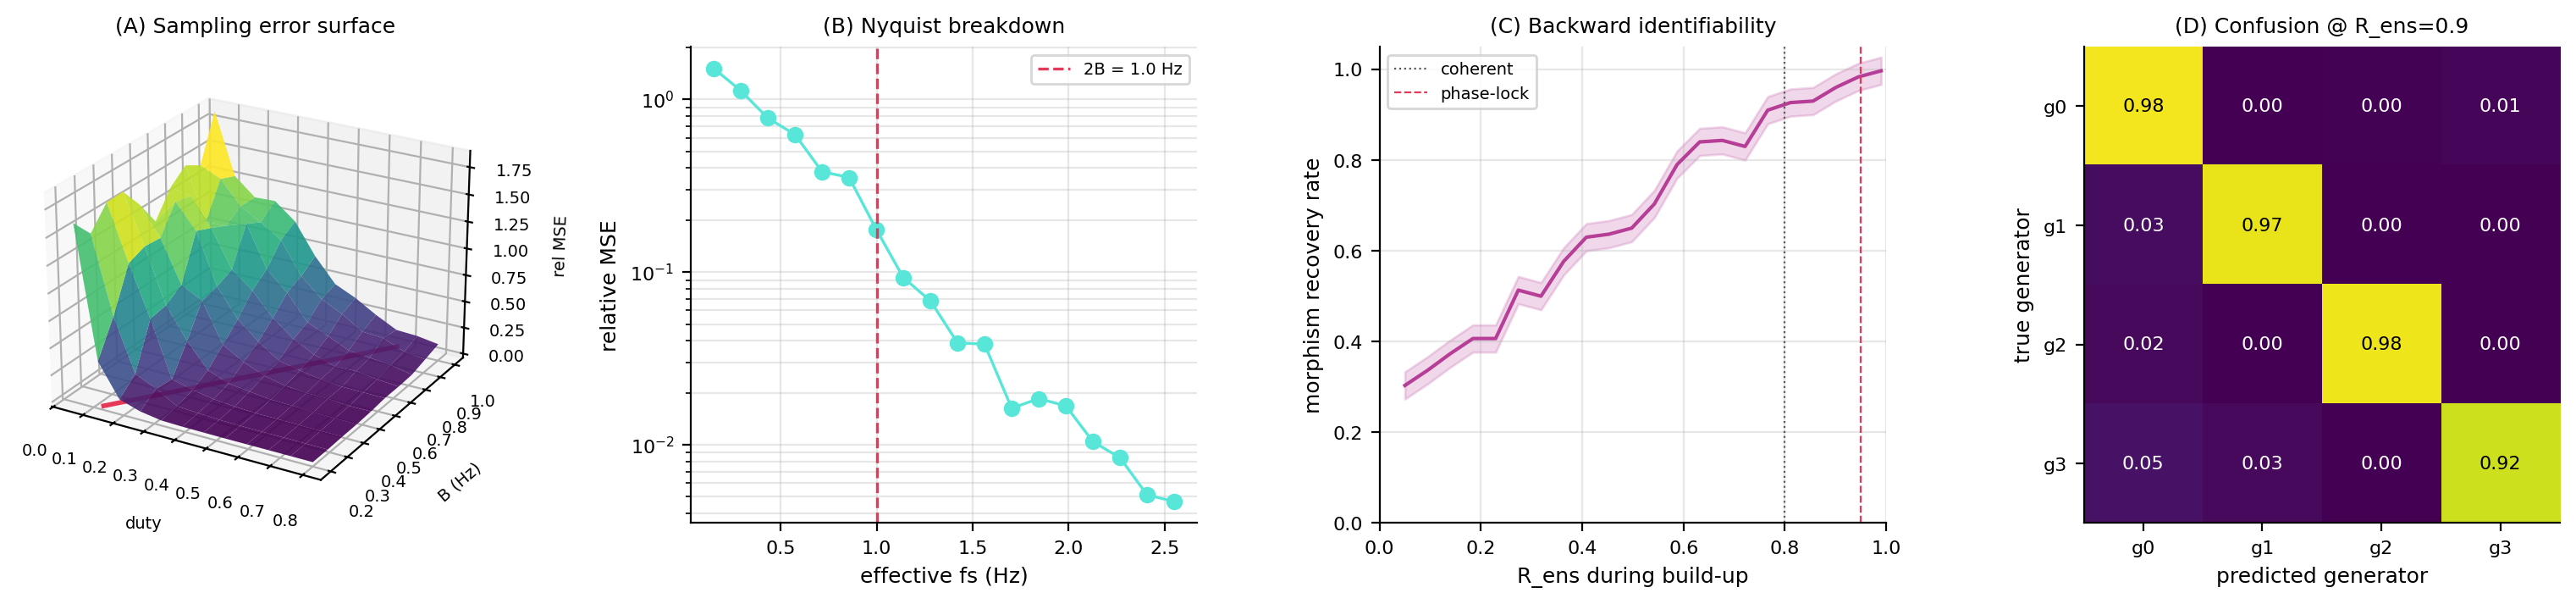
\includegraphics[width=\textwidth]{figures/panel5_sampling_recovery.png}
    \caption{\textbf{Cellular sampling and backward morphism
    identifiability.}
    (\textbf{A})~Three-dimensional surface of relative reconstruction
    MSE over the joint parameter space (duty fraction, signal
    bandwidth) for a player sampled by the ball channel at cadence
    $3$~Hz. The red curve traces the Nyquist boundary $f_{s}=2B$
    (equivalently $\mathrm{duty}=2B/\mathrm{cadence}$) projected onto
    the $z=0$ plane. The surface is high in the sub-Nyquist corner
    (low duty, high bandwidth) and falls toward zero across the
    super-Nyquist region.
    (\textbf{B})~Relative MSE versus effective sample rate $f_{s}$
    (in Hz, log-scale on $y$). The reconstruction error drops by more
    than two orders of magnitude as $f_{s}$ crosses the Nyquist rate
    $2B=1.0$~Hz (red dashed). Sub-Nyquist sampling produces MSE near
    or above unity; super-Nyquist sampling produces MSE near zero.
    (\textbf{C})~Backward morphism recovery rate versus team coherence
    $R_{\mathrm{ens}}$ during build-up. The recovery curve rises
    monotonically from $\sim$35\% at $R_{\mathrm{ens}}=0.10$ (turbulent)
    to $\sim$98\% at $R_{\mathrm{ens}}=0.95$ (phase-locked). The
    vertical lines mark the boundaries of the coherent regime
    (grey dotted, $R=0.80$) and phase-lock (red dashed, $R=0.95$);
    above coherent, the morphism factorisation is identifiable to
    above $85\%$ accuracy.
    (\textbf{D})~Generator confusion matrix at $R_{\mathrm{ens}}=0.9$.
    Rows are true generator labels and columns are the recovered
    label; cell values are conditional probabilities. The diagonal
    dominance ($>0.92$ across all four generators) confirms that
    in the coherent regime the framework correctly identifies which
    of the team's tactical generators executed a given goal build-up,
    with off-diagonal confusion below $5\%$.}
    \label{fig:sampling-recovery}
\end{figure*}
